\documentclass[12pt, a4paper]{article}

\usepackage{amsmath}
\usepackage{amssymb}
\usepackage{booktabs}
\usepackage{graphicx}
\usepackage{caption}
\usepackage{geometry}
\usepackage{hyperref}
\usepackage{siunitx}
\usepackage{array}
\usepackage{float}
\usepackage{setspace}
\usepackage{circuitikz}
\usetikzlibrary{positioning}

\onehalfspacing

\geometry{margin=2.5cm}

\hypersetup{
    colorlinks=true,
    linkcolor=blue,
    urlcolor=blue,
    citecolor=blue
}

\sisetup{per-mode=symbol}

\title{10-bit SAR ADC Design in Sky130 -- Project Report}
\author{}
\date{}

\begin{document}

\maketitle
\tableofcontents
\newpage

% ─────────────────────────────────────────────
\section{Introduction and Specifications}
\label{section:intro}
The successive-approximation (SAR) ADC is the most commonly deployed topology of analog-to-digital converter. Owing to its low power consumption, 
low latency and compact form factor, it has proven supremely versatile, with notable usage in IoT devices, medical equipment and microcontrollers. This document describes an original 10-bit SAR ADC designed and verified in the 
SkyWater Sky130 open-source 130nm process --- a CMOS PDK developed by SkyWater Technology and Google, providing full device model access without NDA --- targeting 
the specifications in Table~\ref{tab:specs}. The design covers the complete front-end flow: behavioral modeling from first principles, transistor-level 
schematic capture in xschem, ngspice simulation against Sky130 device models, and Verilog RTL synthesized to Sky130 standard cells via Yosys. Physical layout 
is out of scope; the project targets schematic-level verification.

\begin{table}[H]
    \centering
    \caption{Design Specifications}
    \label{tab:specs}
    \begin{tabular}{@{}ll@{}}
        \toprule
        Parameter & Value  \\
        \midrule
        Resolution & 10 bits \\
        Sample Rate & 1 $\frac{\text{MS}}{\text{s}}$ \\ 
        ENOB & $\geq$ 9 bits \\
        Supply Voltage, $V_{DD}$ & $\qty{1.8}{V}$ \\
        Reference Voltage, $V_{ref}$ & $\qty{1.8}{V}$ \\
        Input Range & $0\,-\qty{1.8}{V}$ \\
        Process & SkyWater Sky130, 130nm \\
        \bottomrule
    \end{tabular}
\end{table}

The design followed a bottom-up flow, progressing sequentially through each of the following stages:
\begin{enumerate}
    \item First-principles sizing and yield analysis via Python behavioral model
    \item Block-level schematic capture in xschem and isolation verification in ngspice
    \item Verilog RTL synthesis to Sky130 standard cells via Yosys
    \item Full-ADC SPICE integration and static performance characterisation
\end{enumerate}

This document reports the design decisions, block-level verification, integration debugging and static characterisation of the 10-bit SAR ADC. Ultimately, the design achieves a static ENOB of 7.27 bits, falling short of its 9-bit target, attributable to a characterised top-plate feedthrough mechanism, detailed in Section~\ref{sec:integration}..

% ─────────────────────────────────────────────
\section{Architecture Overview}
\label{section:architecture}

The design is comprised of four major blocks: the bootstrapped switch, CDAC binary-weighted array, StrongARM comparator and SAR logic block. 
During the sampling phase, the bootstrapped switch connects $V_{in}$ to all 
bottom plates of the CDAC array simultaneously, while the top plate is reset 
to $V_{cm} = V_{ref}\, /\,2$. This establishes a charge 
on the top plate node of $Q = (V_{ref}/2 - V_{in}) \cdot C_{total}$. At the 
start of conversion, the bootstrapped switch is disconnected, leaving the top plate floating with its charge preserved
while the bottom plate of each node is shorted to ground. The SAR 
logic then performs a binary search from the MSB downward: each trial bit 
steers its corresponding bottom plate to $V_{ref}$, shifting $V_{DAC}$ upward 
by an amount proportional to that capacitor's weight. The StrongARM comparator 
evaluates whether $V_{DAC}$ has crossed $V_{ref}/2$, equivalent to testing whether $V_{in}$ exceeds the 
analog value of the current trial code. The SAR logic retains or clears each 
bit accordingly:

\begin{enumerate}
    \item Assert trial code $1000000000$; bottom plate of $512C$ switches to 
    $V_{ref}$, shifting $V_{DAC}$ upwards.
    \item If $V_{DAC} < V_{ref}/2$ (equivalently, $V_{in} > V_{ref}/2$), 
    retain bit 9; otherwise clear it and return that bottom plate to ground
    \item Assert the next trial bit and repeat in descending order until all 
    10 bits are resolved
\end{enumerate}

This process is summarized by the block diagram in figure~\ref{fig:block_diagram}.

\begin{figure}[H]
    \centering
    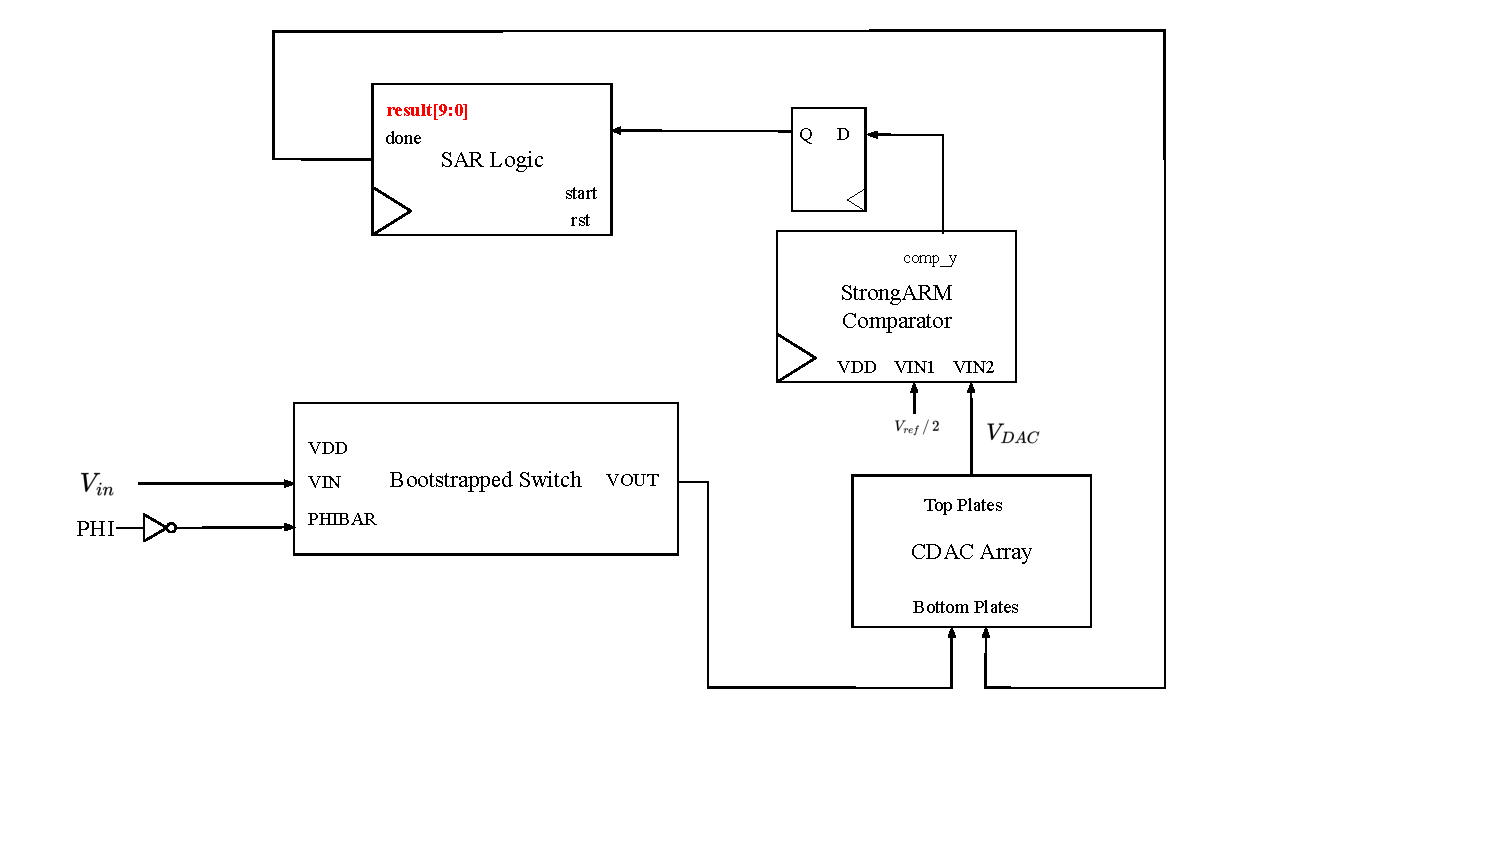
\includegraphics[width=1.1\textwidth]{figures/block_diagram}
    \caption{Block diagram of SAR ADC}
    \label{fig:block_diagram}
\end{figure}

% ─────────────────────────────────────────────
\section{Block Design and Sizing}
\label{section:block_design}

% ─────────────────────────────────────────────
\subsection{Python Behavioral Model}
\label{subsection:behavioral_model}

The minimum valid unit capacitance, $C_{unit}$, that can be used for any capacitor in the CDAC array is governed by the thermal noise floor in equation~\ref{eq:thermal_noise_floor}.

\begin{equation}
    C_{min} = \frac{kT}{V_{LSB}^2} \label{eq:thermal_noise_floor}
\end{equation}

with $V_{LSB} = \frac{V_{ref}}{2^N}$, where $N$ is the resolution of the instrument. Substituting $k = \qty{1.38e-23}{J \cdot K}$, $T = \qty{300}{K}$, $V_{ref} = \qty{1.8}{V}$ and $N=10$,
$C_{min} $ is found as $\qty{5.36}{\femto F}$.

In order to determine a suitable unit capacitance, a Monte Carlo mismatch analysis was conducted. In each trial, $C_{unit}$ was swept from $\qty{5}{fF}$ to $\qty{54}{fF}$ and a binary-weighted capacitor array,
$[512, 256, 128, ..., 2, 1, 1] \times C_{unit}$ was generated, representing the CDAC array. Each capacitor in this array was perturbed according to $\sigma_{C/C} \, / \, \sqrt{n_{cells}}$,
where the mismatch $\sigma_{C/C}$ is 2\%, and $n_{cells} = C_{unit} \, / \, C_{min}$. Using this representation of the CDAC array, the SAR conversion algorithm was executed on $2^{16} = 65\,536$
input voltages, 64 per binary code. For each trial, the DNL and INL were computed and the maximum INL was recorded. This process was repeated for 10\,000 trials.

The yield is computed as the fraction of trials where the maximum INL is less than 0.5 LSB. As can be seen in figure~\ref{fig:yield_vs_cunit}, the yield surpasses its target of 99\%
at approximately $\qty{24}{fF}$. Therefore, to allow for some margin, a target value of $C_{unit} = \qty{25}{fF}$ was selected, giving a total CDAC capacitance of $1024 \times \qty{25}{fF} = \qty{25.6}{pF}$.

\begin{figure}[H]
    \centering
    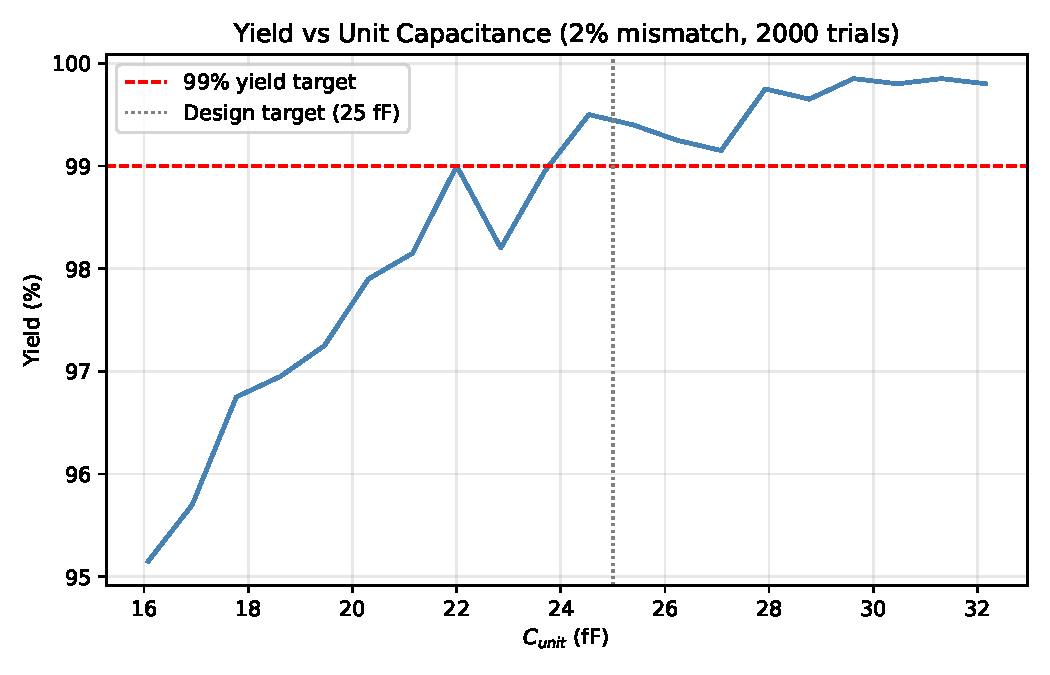
\includegraphics[width=0.75\textwidth]{figures/yield_vs_cunit.pdf}
    \caption{Yield vs.\ $C_{unit}$ sweep across 10\,000 Monte Carlo trials at $\sigma_{C/C} = 2\%$.}
    \label{fig:yield_vs_cunit}
\end{figure}

To validate the selected $C_{unit} = \qty{25}{fF}$, a further 10\,000-trial Monte Carlo simulation was run at this fixed value. Figure~\ref{fig:monte_carlo_histogram} shows the resulting distribution
of maximum INL across all trials. The distribution is centred near $\qty{0.2}{LSB}$, with a tail that barely reaches the $\qty{0.5}{LSB}$ threshold, confirming a yield of 99.2\%.

\begin{figure}[H]
    \centering
    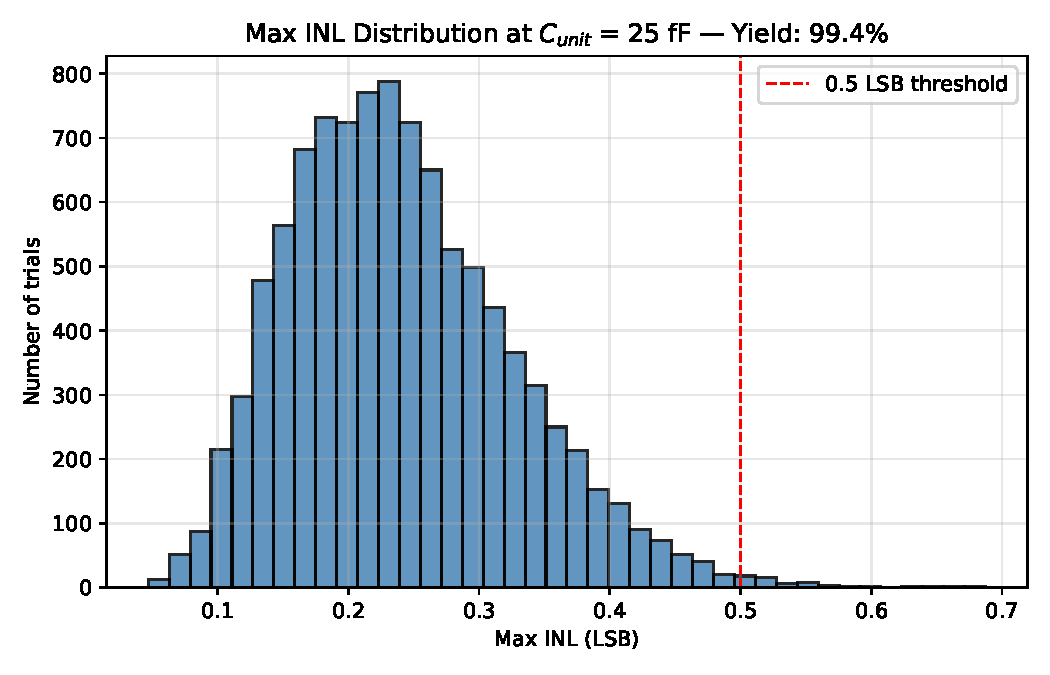
\includegraphics[width=0.75\textwidth]{figures/monte_carlo_histogram.pdf}
    \caption{Distribution of maximum INL at $C_{unit} = \qty{25}{fF}$, 10\,000 Monte Carlo trials, $\sigma_{C/C} = 2\%$. Yield: 99.2\%.}
    \label{fig:monte_carlo_histogram}
\end{figure}

Figure~\ref{fig:dnl_inl_example} shows the DNL and INL of a representative single trial at $C_{unit} = \qty{25}{fF}$. The DNL remains well within $\pm 0.5\,\text{LSB}$ across all 1024 output codes,
with no missing codes. The INL exhibits a random-walk character, as expected from independent capacitor mismatch errors accumulating across the code range, and stays within $\pm 0.5\,\text{LSB}$ throughout.

\begin{figure}[H]
    \centering
    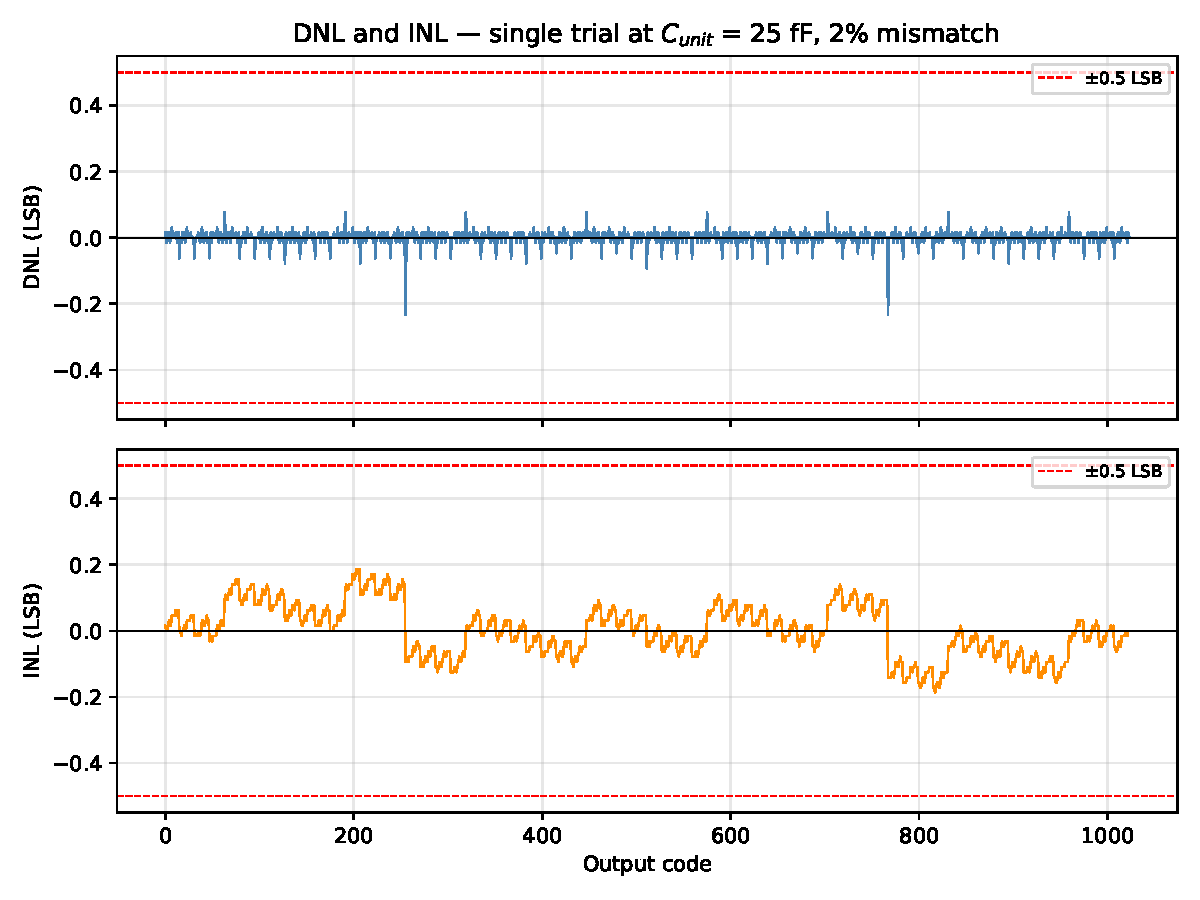
\includegraphics[width=0.75\textwidth]{figures/dnl_inl_example.pdf}
    \caption{DNL and INL for a single representative trial at $C_{unit} = \qty{25}{fF}$, $\sigma_{C/C} = 2\%$.}
    \label{fig:dnl_inl_example}
\end{figure}

% ─────────────────────────────────────────────
\subsection{CDAC}
\label{subsection:cdac}

The CDAC is a binary-weighted array of capacitors, $[512, 256, 128, ..., 2, 1, 1] \times C_{unit}$. Including the termination capacitor of capacitance 
$C_{unit}$, it spans 11 capacitors with a total capacitance of $1024 \cdot C_{unit} = \qty{25.6}{pF}$. The top plate of each capacitor is tied to the common node $V_{DAC}$,
while each capacitor has a unique bottom plate node. 
During operation, the CDAC undergoes two stages:

\begin{enumerate}
    \item Sampling: the bottom plate of each capacitor is driven to $V_{in}$, while $V_{DAC}$ is driven to $V_{cm} = V_{ref} \, / \, 2$. This locks in a charge of $Q = 1024 \cdot C_{unit} \cdot (V_{ref} \, / \, 2 - V_{in})$ onto the CDAC.
    \item Conversion: $V_{DAC}$ is disconnected from its source and becomes floating. The SAR logic block drives the bottom plate of each capacitor to either $V_{ref}$ or ground, depending on whether the corresponding bit in the code under trial is high or low. For example, if the code under trial is $1010000000$, then the bottom plates of $C_9 = 512 C_{unit}$ and $C_7 = 128 C_{unit}$ are sent to $V_{ref}$, with the remaining bottom plates being shorted to ground. At the end of conversion, $V_{DAC} = \frac{W}{1024} V_{ref} + V_{ref} \, / \, 2 - V_{in}$, where $W$ is the sum of the weights of each capacitor whose bottom plate is at $V = V_{ref}$. Note that during conversion, the bottom plate of the termination capacitor is always shorted to ground.
\end{enumerate}

For each analog voltage under test, sampling occurs once at the start of the procedure, while conversion happens once per bit, progressing from the MSB to the LSB. 
The transistor-level logic that controls the CDAC's behavior is shown in figure~\ref{fig:cdac_cell}.

\begin{figure}[h]
\centering
\begin{circuitikz}[scale=1.0, transform shape, every node/.style={font=\small}]
 
% ── top-plate reset TG ──────────────────────────────────────
\node[tgate, scale=0.8] (tgtop) at (2.5, 8.0) {};
\node[above, font=\footnotesize] at (tgtop.north) {$\phi_s$};
\node[below, font=\footnotesize] at (tgtop.south) {$\bar{\phi}_s$};
\node[left,  font=\footnotesize] at (tgtop.in) {$V_{cm}$};
 
% vdac node
\coordinate (vdac) at (4.5, 8.0);
\node[circ] at (vdac) {};
\node[above, font=\footnotesize] at (vdac) {$V_{DAC}$};
\draw (tgtop.out) -- (vdac);
 
% vdac down wire + cap
\draw (vdac) -- (4.5, 6.8);
\draw (4.5, 6.8) to[C, l_=$C_N$] (4.5, 5.2);
\coordinate (bpN) at (4.5, 5.2);
\node[circ] at (bpN) {};
\node[below right, font=\footnotesize] at (bpN) {$bp_N$};
 
% ── PMOS ref switch (above bpN, right side) ──────────────────
\node[pmos, scale=0.8, xscale=-1] (pref) at (7.0, 6.5) {};
\draw (pref.source) -- ++(0, 0.5) node[above, font=\footnotesize] {$V_{ref}$};
\draw (pref.drain) -- (7.0, 5.2) -- (bpN);
\draw (pref.gate) -- ++(0, 0) node[right, font=\footnotesize] {$\overline{\mathit{cdac\_sw}}_N$};

% ── sample TG ────────────────────────────────────────────────
\node[tgate, scale=0.8] (tgsmp) at (2.5, 5.2) {};
\node[above, font=\footnotesize] at (tgsmp.north) {$\phi_s$};
\node[below, font=\footnotesize] at (tgsmp.south) {$\bar{\phi}_s$};
\node[left,  font=\footnotesize] at (tgsmp.in) {$V_{in,s}$};
\draw (tgsmp.out) -- (bpN);
 
% ── NMOS gnd1 ────────────────────────────────────────────────
\node[nmos, scale=0.8] (gnd1) at (4.5, 3.8) {};
\draw (gnd1.drain) -- (bpN);
\draw (gnd1.gate) -- ++(-0.4, 0) node[left, font=\footnotesize] {$\overline{\mathit{cdac\_sw}}_N$};
 
% ── NMOS gnd2 ────────────────────────────────────────────────
\node[nmos, scale=0.8] (gnd2) at (4.5, 2.3) {};
\draw (gnd2.drain) -- (gnd1.source);
\draw (gnd2.source) node[ground] {};
\draw (gnd2.gate) -- ++(-0.4, 0) node[left, font=\footnotesize] {$\bar{\phi}_s$};
 
\end{circuitikz}
\caption{Transistor-level design of one CDAC cell}
\label{fig:cdac_cell}
\end{figure}

The diagram in figure~\ref{fig:cdac_cell} applies to all capacitors in the CDAC except for the termination capacitor. Note that for compactness, the transmission gate responsible for charging $V_{DAC}$ to
$V_{cm}$ during sampling is included in figure~\ref{fig:cdac_cell}; however, because $V_{DAC}$ is shared by all capacitors, the entire CDAC only uses one such transmission gate rather than one per cell. 
The signal $cdac\_sw_N$ represents the high/low value of $N^{th}$ trial bit in the code under test. The capacitor $C_{N}$ is responsible for the voltage contribution of this bit to $V_{DAC}$, and has a capacitance
value of $C_N = 2^N \cdot C_{unit}$.

During sampling, $\phi_s$ is high, meaning that both transmission gates are active and $V_{DAC}$ gets sent to $V_{cm}$ while each $V_{bp_N}$ is sent to $V_{in}$. 
Thereafter, $\phi_s$ turns off and both transmission gates are switched off, leaving $V_{DAC}$ floating and initiating the conversion stage. If $cdac\_sw_N$ is high, then its complement $\overline{\mathit{cdac\_sw}}_N$ is low and the PMOS of the
pull-up network turns on, shorting $bp_N$ to $V_{ref}$. Otherwise, the top NMOS in the pull-down network is activated and $bp_N$ is routed to ground. The additional NMOS gated by $\bar{\phi}_s$ in the pull-down
network is introduced due to contention; if it were not there, then the pull-down network would provide a path to ground during sampling while $cdac\_sw_N$ is low. Since $\phi_s$ is guaranteed to be high during sampling and low during conversion, this NMOS ensures that the pull-down network is never active during sampling but can still be active during conversion.

Note that due to its repetitive nature, no schematic for the CDAC array was designed by hand, with cdac.spice instead being written directly.

% ─────────────────────────────────────────────
\subsection{Bootstrapped Switch}
\label{subsection:bootstrapped_switch}

Bootstrapping is necessary in order to avoid bandwidth modulation and harmonic distortion when charging the bottom plates of the CDAC up to $V_{in}$. When an NMOS is used to charge up the CDAC,
the channel resistance $R_{on}$ of the FET and the capacitance of the CDAC create a low-pass filter with cutoff frequency given by equation~\ref{eq:cutoff_frequency}.

\begin{equation}
    f_n = \frac{1}{2\pi R_{on} C_{DAC}} \label{eq:cutoff_frequency}
\end{equation}

The channel resistance $R_{on}$ of an NMOS is given by equation~\ref{eq:nmos_resistance}.

\begin{equation}
    R_{on} = \frac{1}{\mu_n C_{ox} \frac{W}{L} (V_{GS} - V_{th,n})} \label{eq:nmos_resistance}
\end{equation}

If the FET is gated by $V_{DD}$, then $V_{GS} = V_{DD} - V_{in}$, meaning that if $V_{in}$ changes, the bandwidth of the low-pass filter varies, attenuating signals inconsistently.
This unevenness results in harmonic distortion, lowering the effective resolution of the instrument. The bootstrapped switch combats this by lifting the gate voltage of the FET to $V_{DD} + V_{in}$, therefore 
fixing $V_{GS}$ at $V_{DD}$, thus fixing $R_{on}$ and the corresponding cutoff frequency of the transfer function.

The topology of the bootstrapped switch is shown in figure~\ref{fig:bootstrap}. It operates in two stages.

\begin{enumerate}
    \item When $\phi_s$ is low, the PMOS $Q_2$ is off while the NMOS $Q_5$ is on, therefore wiring the node X to ground. As such, the NMOS's $Q_4$ and $Q_0$ are off, while the PMOS $Q_1$ and the NMOS $Q_3$ are on. Therefore, there is a direct pathway from $V_{DD}$ to ground through $C_{boot}$, which charges up to $V_{DD}$.
\item When $\phi_s$ turns on, transistors $Q_3$ and $Q_5$ turn off while transistor $Q_2$ turns on, allowing $V_X = V_{DD} + V_{in}$. This causes transistor $Q_1$ to turn off and transistors $Q_4$ and $Q_0$ to turn on, thus providing a pathway for $V_{in}$ to flow into $V_{in,s}$ with the gate of $Q_0$ fixed at $V_X$.
\end{enumerate}

\begin{figure}[h]
\centering
\begin{circuitikz}[american, scale=0.9, transform shape]

% --- Q0: NMOS drain=VIN, gate=X, source=VIN_S ---
  \node[nmos, rotate=-90] (Q0) at (4,2) {};
  \draw (Q0.drain) -- (5,2) node[right] {$V_{in,s}$};
  \filldraw[white] (Q0.drain) circle (2pt);
  \draw (Q0.drain) circle (2pt);
  \draw (Q0.gate) -- (4,3) -- (4,4);
  \draw (Q0.source) -- ++(0,-0.7);
  \filldraw[white] (Q0.source) ++(0,-0.7) circle (2pt);
  \draw (Q0.source) ++(0,-0.7) circle (2pt) node[below=2pt] {$V_{in}$};
  \node[below] at (4,1.5) {$Q_0$};

  % --- Q1: PMOS drain=VDD, gate=X, source=net3 ---
  \node[pmos, rotate=-90] (Q1) at (0,6) {};
  \draw (Q1.drain) -- (-1,6) -- (-1,6.5) node[above] {$V_{DD}$};
  \draw[->, >=latex] (-1,6) -- (-1,6.5);
  \draw (Q1.gate)  -- (0,7) node[above] {$X$};
  \node[below] at (0,5.5) {$Q_1$};
  
  % --- Q2: PMOS drain=net3, gate=PHIBAR, source=X ---
  \node[pmos, rotate=-90] (Q2) at (2,6) {};
  \draw (Q2.gate)  -- (2,7) node[above] {$\bar{\phi_s}$};
  \node[below] at (2,5.5) {$Q_2$};

  % net3 wire: Q1 source to Q2 drain
  \draw (Q1.source) -- (Q2.drain);

  % --- Q3: NMOS drain=net2, gate=PHIBAR (points DOWN), source=GND ---
  \node[nmos, rotate=90] (Q3) at (0,2) {};
  \draw (Q3.drain) -- (-1,2) node[ground] {};
  \draw (Q3.gate)   -- (0,1) node[below] {$\bar{\phi_s}$};
  \node[above] at (0,2.5) {$Q_3$};

  % --- Q4: NMOS drain=net2, gate=X, source=VIN ---
  \node[nmos, rotate=-90] (Q4) at (2,2) {};
  \draw (Q4.drain)  -- (Q0.source);
  \draw (Q4.source) -- (Q3.source);
  \draw (Q4.gate)   -- (2,3);      % gate up to X bus
  \node[below] at (2,1.5) {$Q_4$};

% C_boot: top plate at Q1.source, bottom plate at Q3/Q4 source level
  \draw (Q1.source) to[C, l_=$C_{boot}$, *-*] (Q3.source);
  \filldraw (Q1.source) circle (1.5pt);
  \filldraw (Q3.source) circle (1.5pt);

  % --- X bus at y=4 (horizontal) ---
  \draw (4,4) -- (2,4);
  \node[below] at (3,4) {$X$};
  \filldraw (3,4) circle (1.5pt);
  % Q4 gate up to X
  \draw (2,3) -- (2,4);
  % Q2 source to X
  \draw (Q2.source) -- (3,6) -- (3,4);

  % --- Q5: NMOS drain=X, gate=PHIBAR, source=GND ---
  \node[nmos, rotate=-90] (Q5) at (4,6) {};
  \draw (Q5.source)  -- (3,6);      % drain left to X
  \draw (Q5.drain) -- (5,6) node[ground] {};
  \draw (Q5.gate)   -- (4,7) node[above] {$\bar{\phi_s}$};
  \node[below] at (4,5.5) {$Q_5$};

\end{circuitikz}
\caption{Bootstrapped sampling switch. $Q_0$ is the main sampling device;
$C_{boot}$ is precharged to $V_{DD}$ during $\bar{\phi_s}$ and
bootstraps the gate of $Q_0$ to $V_{in}+V_{DD}$ during $\phi_s$.}
\label{fig:bootstrap}
\end{figure}

Together with the CDAC, the bootstrapped switch enforces the three-phase behavior of the signal $\phi_s$. 
During phase 1, $\phi_s$ must be low so as to allow $C_{boot}$ to charge. Then, $\phi_s$ must become high to turn the switch on and charge up the CDAC.
Finally, $\phi_s$ permanently turns off, disconnecting the CDAC from the bootstrapped switch which has accomplished its purpose by fixing charge onto the CDAC.

In totality, this means that $\phi_s$ must be a pulse which must start at a delay. The length of this pulse determines the sizing of the transistors and the value
of $C_{boot}$. This length, in turn, is determined by the sample rate design target, 1 megasample per second.

A rate of 1 megasample per second implies a period of $\qty{1}{\mu s}$. Using a typical 70-30 split, with 30\% of the period allotted to sampling, the width of the pulse
is $\qty{300}{ns}$. During the width of this pulse, the CDAC must be charged up enough to render an error due to rounding impossible. Practically, this means that the error
of the CDAC's voltage must be less than half of an LSB. The error of the CDAC's voltage, defined as the difference between $V_{in}$ and $V_{DAC}$, is given by equation~\ref{eq:cdac_error}.

\begin{equation}
    \text{Error} = V_{in} \cdot e^{-t \, /  \, R_{on} C_{DAC}} \label{eq:cdac_error}
\end{equation}

Requiring this error to be less than the value of half of one LSB, $\text{Error} < \frac{V_{ref}}{2^{N+1}}$, and assuming a worst-case scenario of $V_{in} = V_{ref}$, an expression for $R_{on}$ can be derived.

\begin{equation}
    R_{on} \le \frac{t}{C_{DAC} \cdot 2^{N+1} \cdot \ln 2}
\end{equation}

Substituting $t = \qty{300}{ns}$, $C_{DAC} = \qty{25.6}{pF}$ and $N = 10$, $R_{on}$ is found as $\qty{1.54}{\kilo \Omega}$. Applying the channel resistance equation of equation~\ref{eq:nmos_resistance},
with $V_{GS} = V_{DD} = \qty{1.8}{V}$ due to bootstrapping, $\mu_n C_{ox} = \qty{270}{\frac{\mu A}{V^2}}$ as set by Sky130, and $l = \qty{150}{nm}$ (the minimum allowable channel length in Sky130),
the minimum value for $w$ is found as $\qty{273.8}{nm}$. Allowing for an ample margin, the transistor $Q_0$ was chosen to have a width of $\qty{1}{\mu m}$. Auxiliary transistors $Q_1$ and $Q_{3-5}$ were sized to match $Q_0$'s width layout for convenience,
while $Q_2$ was sized conservatively with a width double that of $Q_0$. All transistors have an identical length of $\qty{150}{nm}$.


Using these design parameters, a value of $C_{boot}$ was selected that sufficiently minimizes droop. 
The voltage droop on $C_{boot}$ due to charge sharing with the parasitic gate capacitance of $Q_0$, $C_{gate}$, is given by equation~\ref{eq:droop}.

\begin{equation}
    \frac{\Delta V}{V_{DD}} = \frac{C_{gate}}{C_{gate} + C_{boot}} \label{eq:droop}
\end{equation}

Setting this quantity to be strictly less than 0.01,

\begin{gather}
    \frac{C_{gate}}{C_{gate} + C_{boot}} < 0.01 \nonumber \\
    100 \cdot C_{gate} < C_{boot} + C_{gate} \nonumber \\
    \boxed{C_{boot} > 99 \cdot C_{gate}} \label{eq:c_boot}
\end{gather}

The gate capacitance, $C_{gate}$, is given by $C_{gate} = wl \cdot C_{ox}$. Substituting $w = \qty{1}{\mu m}$, $l = \qty{150}{nm}$ and $C_{ox} = \qty{17}{\frac{fF}{\mu m^2}}$ as set by Sky130,
$C_{boot} > \qty{252.45}{fF}$. To significantly exceed this mark, $C_{boot}$ was chosen as $\qty{500}{fF}$. The final design choices are summarized in table~\ref{tab:sizing}.

\begin{table}[H]
    \centering
    \caption{Sizing Choices}
    \label{tab:sizing}
    \begin{tabular}{@{}ll@{}}
        \toprule
        Parameter & Value  \\
        \midrule
        Width of $Q_0$ & $\qty{1}{\micro m}$ \\
        Channel length of $Q_0$ & $\qty{150}{nm}$ \\ 
        $C_{boot}$ & $\qty{500}{fF}$ \\
        \bottomrule
    \end{tabular}
\end{table}

% ─────────────────────────────────────────────
\subsection{StrongARM Comparator}
\label{subsection:strongarm_comparator}

The StrongARM comparator is the block which performs the bitwise retain or reject decision making for each trial code. Its topology is shown in figure~\ref{fig:strongarm_comparator}.

\begin{figure}[H]
\centering
\begin{circuitikz}[american, font=\small, scale=0.85, transform shape]
 
%--- VDD rail ---
\draw (-4.5,10.5) -- (4.5,10.5) node[right]{$V_\mathrm{DD}$};

%% M7 — tail NMOS
\node[nmos, anchor=source] (M7) at (0,2) {};
\draw (M7.gate) -- ++(-0.8,0) node[left]{CLK};
\node[right=3pt] at (M7.east) {$M_7$};

%% M1 — left input NMOS
\node[nmos, anchor=source] (M1) at (-1.3,3.542) {};
\draw (M1.gate) -- ++(-0.8,0) node[left]{$V_{in1}$};
\node[right=3pt] at (M1.east) {$M_1$};
\draw (M1.source) -- (0,3.542);

%% M2 — right input NMOS
\node[nmos, xscale=-1, anchor=source] (M2) at (1.3,3.542) {};
\draw (M2.gate) -- ++(0.8,0) node[right]{$V_{in2}$};
\node[left=17pt] at (M2.west) {$M_2$};
\draw (M2.source) -- (0,3.542);

% tail wire
\draw (M7.drain) -- (0,3.542);

% P node: M1 drain meets M3 source
\draw (M1.drain) -- (-1.3,5.1) node[circ]{} node[right]{$P$};

% Q node: M2 drain meets M4 source
\draw (M2.drain) -- (1.3,5.1) node[circ]{} node[left]{$Q$};

% --- M3 NMOS source=P, drain=X, gate=Y ---
\node[nmos, xscale=-1, anchor=source] (M3) at (-1.3,5.1) {};
\node[left=15pt] at (M3.west) {$M_3$};

% --- M4 NMOS source=Q, drain=Y, gate=X ---
\node[nmos, anchor=source] (M4) at (1.3,5.1) {};
\node[right=3pt] at (M4.east) {$M_4$};

% --- M5: PMOS source=VDD, gate=Y, drain=X ---
\node[pmos, xscale=-1, anchor=source] (M5) at (-1.3,10.5) {};
\node[left=16pt] at (M5.gate) {$M_5$};

% --- M6: PMOS source=VDD, gate=X, drain=Y ---
\node[pmos, anchor=source] (M6) at (1.3,10.5) {};
\node[right=16pt] at (M6.gate) {$M_6$};

% X / Y node markers
\draw (-1.3,7.342) node[circ]{} node[right=5pt]{$X$};
\draw (1.3,7.342) node[circ]{} node[left=5pt]{$Y$};

% M5 drain to M3 drain (both at X)
\draw (M5.drain) -- (-1.3,7.342);
\draw (M3.drain) -- (-1.3,7.342);

% M6 drain to M4 drain (both at Y)
\draw (M6.drain) -- (1.3,7.342);
\draw (M4.drain) -- (1.3,7.342);

% Cross-coupled gates: Y to M3 gate, X to M4 gate
\draw (M3.gate) -- (1.3,7.342);
\draw (M4.gate) -- (-1.3,7.342);

% Cross-coupled PMOS gates: M5 gate=Y, M6 gate=X
\draw (M5.gate) -- (1.3,7.342);
\draw (M6.gate) -- (-1.3,7.342);

% --- S3: PMOS drain=X, gate=CLK, source=VDD ---
\node[pmos, anchor=source] (S3) at (-2.5,10.5) {};
\node[right=3pt] at (S3.drain) {$S_3$};
\draw (S3.drain) -- (-2.5,7.342) -- (-1.3,7.342);

% --- S4: PMOS drain=Y, gate=CLK, source=VDD ---
\node[pmos, xscale=-1, anchor=source] (S4) at (2.5,10.5) {};
\node[left=3pt] at (S4.drain) {$S_4$};
\draw (S4.drain) -- (2.5,7.342) -- (1.3,7.342);

% --- S1: PMOS drain=P, gate=CLK, source=VDD ---
\node[pmos, anchor=source] (S1) at (-3.8,10.5) {};
\draw (S1.gate) -- ++(-0.8,0) node[left]{CLK};
\node[right=3pt] at (S1.drain) {$S_1$};
\draw (S1.drain) -- (-3.8,5.1) -- (-1.3,5.1);

% --- S2: PMOS drain=Q, gate=CLK, source=VDD ---
\node[pmos, xscale=-1, anchor=source] (S2) at (3.8,10.5) {};
\draw (S2.gate) -- ++(0.8,0) node[right]{CLK};
\node[left=3pt] at (S2.drain) {$S_2$};
\draw (S2.drain) -- (3.8,5.1) -- (1.3,5.1);

% extend CLK from S1 gate across to S3 gate
\draw (S1.gate) -- (S3.gate);

% extend CLK from S2 gate across to S4 gate
\draw (S2.gate) -- (S4.gate);

\draw (M7.source) node[ground]{};
 
\end{circuitikz}
\caption{StrongARM latch comparator (Figure 1(b) from Razavi \cite{razavi2015strongarm}). M1--M2 form the input differential pair, M3--M4 the cross-coupled NMOS latch, M5--M6 the cross-coupled PMOS latch, M7 the tail switch, and S1--S4 the precharge switches. Nodes P and Q are the intermediate amplification nodes; X and Y are the differential outputs.}
\label{fig:strongarm_comparator}
\end{figure}

When the clock is low, the pull-up network is active and the nodes P, Q, X and Y are pulled up to $V_{DD}$. When the clock turns on, 
the pull-up network is disabled while the NMOS pull-down network comprised of M1, M2 and M7 is enabled, offering a pathway for the voltages at P and Q to discharge to ground. If $V_{in1}$ exceeds $V_{in2}$, the gate-source voltage and hence the rate of discharge at P is
greater than that of Q, and if the reverse is true ($V_{in2} > V_{in1}$), then Q discharges faster than P. Suppose that $V_{in1} > V_{in2}$.
Then, P discharges faster than Q, meaning that the NMOS M3 turns on before M4, offering a discharge pathway to ground for the voltage at X. 
Due to the cross-coupling between M3, M4, M5 and M6, X decreasing means that the gate voltage at M4 decreases, slowing the rate of discharge at Y.
Eventually, $V_X$ is low enough to enable M6 while disabling M4, hence pulling Y up to $V_{DD}$. Therefore, if $V_{in1} > V_{in2}$, $V_Y$ settles at $V_{DD}$
at steady state, while $V_X$ settles at 0. Following identical logic, in the reverse case where $V_{in2} > V_{in1}$, $V_{Y}$ settles at 0 while $V_{X}$ settles at $V_{DD}$.

During operation, $V_{in1} = V_{ref} \, / \, 2$ while $V_{in2} = V_{DAC}$. As noted in subsection~\ref{subsection:cdac}, $V_{DAC} = \frac{W}{1024} V_{ref} + V_{ref} \, / \, 2 - V_{in}$ at the end of conversion. The condition for Y to be high is:

\begin{gather}
    V_{in1} > V_{in2} \nonumber \\
    V_{ref} \, / \, 2 > V_{DAC} \nonumber \\
    V_{ref} \, / \, 2 > \frac{W}{1024} V_{ref} + V_{ref} \, / \, 2 - V_{in} \nonumber \\
    0 > \frac{W}{1024} V_{ref} - V_{in} \nonumber \\
    \boxed{V_{in} > \frac{W}{1024} V_{ref}} \label{eq:comp_eqn}
\end{gather}

Therefore, when Y is high, the trial bit is asserted according to the SAR logic of section~\ref{section:architecture}.

\end{document}